\documentclass[a4paper, 12pt]{article}

\usepackage[left=2cm,right=2cm,
    top=2cm,bottom=2cm,bindingoffset=0cm]{geometry}

\usepackage[T2A]{fontenc}
\usepackage[utf8]{inputenc}
\usepackage{color}
\usepackage{graphicx}
\usepackage{caption}
\usepackage{subcaption}
\usepackage{tikz}
\usepackage[english, russian]{babel}
\usepackage{ gensymb }
\usepackage{booktabs}
\usepackage{amsmath,amsfonts,amssymb,amsthm,mathtools}
\usepackage{lscape}
\usepackage{listings}

\begin{document}


\begin{center}
\textbf{Метод конечных элементов для одномерной задачи теплопроводности с использованием комплекс элементов.}
\end{center}
\begin{center}
\textbf{\textit{Задание}}
\end{center}

Определить распределение температуры в стержне кругового сечения с граничными условиями 1 рода на левой границе стержня и граничными условиями 3 рода на правой границе стержня и на боковой поверхности с использованием квадратичного и кубического одномерного конечного элемента. Сравнить с аналитическим решением.

\begin{center}
    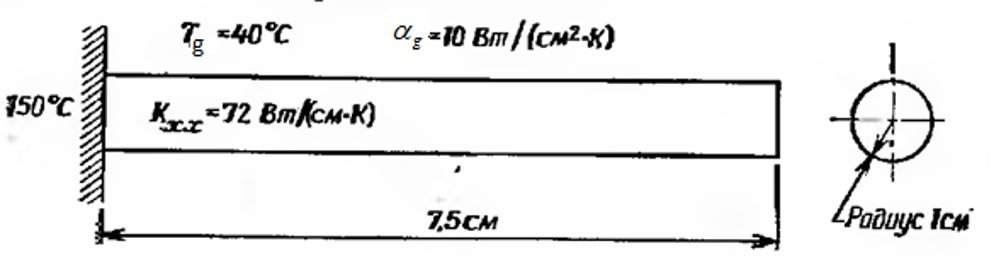
\includegraphics[scale=0.5]{task.jpeg}
\end{center}

\begin{center}
    \textbf{\textit{Решение}}
\end{center}

\begin{enumerate}
    \item Проведем дискретизацию области одномерными элементами для квадратичного и кубического элементов:
    \begin{enumerate}
        \item Схема разбиения области для квадратичного элемента:
        \begin{center}
            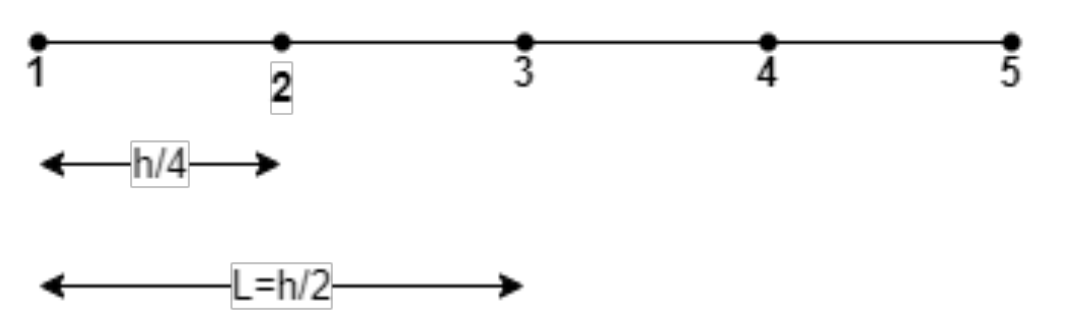
\includegraphics[scale=0.3]{square.png}
        \end{center}
        
        \item Схема разбиения области для кубического элемента:
        \begin{center}
            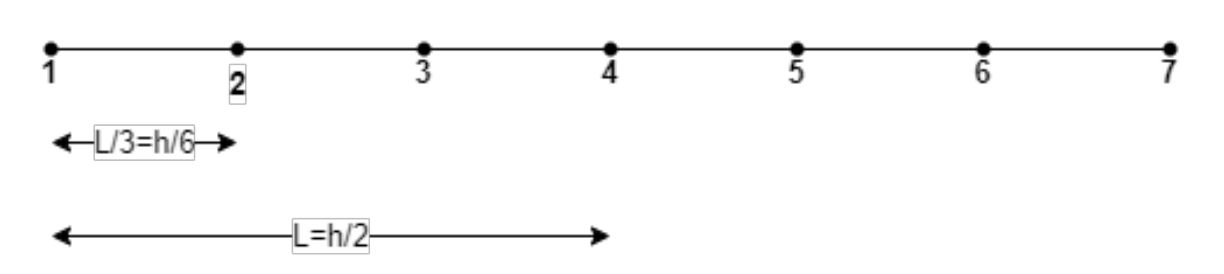
\includegraphics[scale=0.3]{cube.png}
        \end{center}
    \end{enumerate}

    \newpage
    \item Процедура формирования локальных и глобальной матриц
    теплопроводности

    Для расчёта локальных матриц используем приведённые выше формулы.

    Заметим, что бесконечно малые элементы в силу равномерного
    распределения температуры в поперечном сечении и равномерном
    действии ГУ по периметру поперечного сечения можно представить в
    виде \(dV = \pi R^2 dx\) и \(dS = 2\pi R dx\). Дальше требуется лишь вычислить
    две локальные матрицы жёсткости и два вектора правых частей.

    Глобальная матрица составляется следующим образом: первую
    локальную матрицу записываем в элементы глобальной матрицы с 1-3
    столбцы и строки, вторую в 3-5 строки и столбцы соответственно, но к
    элементу глобальной матрицы (3,3) прибавляем элемент (1,1) второй
    локальной матрицы.

    При формировании глобальной матрицы учтём ГУ \(T_1 = 150\) Для
    этого обнулим внедиагональные элементы в строках 1, а диагональные
    положим равными единице.

    \item Код программы, реализующий вычисления:
    
    \begin{lstlisting}[language=Python]
import numpy as np
import matplotlib.pyplot as plt
from sympy import symbols, Matrix, integrate, pi

T_1 = 150
a_g = 10
T_g = 40
lambda_ = 72
H = 7.5
L = H / 2

T_anal = np.array([150, 80.9, 55.4, 46.2, 43.3])
X_anal = np.array([0, L/2, L, 3*L/2, 2*L])
R = 1
S = pi * R**2
P = 2 * pi * R

# First element
X = np.array([0, L])
len_X = len(X)
x = symbols('x')
N = Matrix.zeros(len_X, 3)

for i in range(len_X):
    N[i, 0] = (x - X[i] - L/2) * 
        (x - X[i] - L) / ((-L/2) * (-L))
    N[i, 1] = (x - X[i]) * (x - X[i] - L) / ((L/2) * (-L/2))
    N[i, 2] = (x - X[i]) * (x - X[i] - L/2) / (L * (L/2))

B = N.diff(x)
K_e = np.zeros((3, 3, 2))
f_e = np.zeros((3, 1, 2))

for i in range(len_X):
    K_e[:, :, i] = integrate(S * B[i, :].T * lambda_ * B[i, :], 
        (x, X[i], X[i] + L)) + \
        integrate(P * a_g * N[i, :].T * N[i, :], (x, X[i], X[i] + L))
    f_e[:, 0, i] = integrate(P * a_g * T_g * N[i, :], 
        (x, X[i], X[i] + L))

# Global matrix formation
K = np.zeros((5, 5))
F = np.zeros((5, 1))

K[0:3, 0:3] = K_e[:, :, 0]
K[3:5, 3:5] = K_e[1:3, 1:3, 1]

F[0:3, 0] = f_e[:, 0, 0]
F[3:5, 0] = f_e[1:3, 0, 1]

F[2, 0] += f_e[0, 0, 1]

K[2, 2] += K_e[0, 0, 1]
K[2, 3] += K_e[0, 1, 1]
K[2, 4] += K_e[0, 2, 1]
K[3, 2] += K_e[1, 0, 1]
K[4, 2] += K_e[2, 0, 1]

K[0, 0] = 1
K[0, 1:5] = 0
F[0, 0] = T_1

T = np.linalg.solve(K, F)

# Second element
L = H / 2
X = np.array([0, L])
len_X = len(X)
N = Matrix.zeros(len_X, 4)

for i in range(len_X):
    N[i, 0] = (x - X[i] - L/3) * (x - X[i] - 2*L/3) 
        * (x - X[i] - L) / ((-L/3) * (-2*L/3) * (-L))
    N[i, 1] = (x - X[i]) * (x - X[i] - 2*L/3) * 
        (x - X[i] - L) / ((L/3) * (-L/3) * (-2*L/3))
    N[i, 2] = (x - X[i]) * (x - X[i] - L/3) * 
        (x - X[i] - L) / (2*L/3 * (L/3) * (-L/3))
    N[i, 3] = (x - X[i]) * (x - X[i] - L/3) * 
        (x - X[i] - 2*L/3) / (L * (2*L/3) * (L/3))

B = N.diff(x)
K_e = np.zeros((4, 4, 2))
f_e = np.zeros((4, 1, 2))

for i in range(len_X):
    K_e[:, :, i] = integrate(S * B[i, :].T * lambda_ * B[i, :], 
        (x, X[i], X[i] + L)) + \
        integrate(P * a_g * N[i, :].T * N[i, :], (x, X[i], X[i] + L))
    f_e[:, 0, i] = integrate(P * a_g * T_g * N[i, :], 
            (x, X[i], X[i] + L))

# Global matrix formation
K = np.zeros((7, 7))
F = np.zeros((7, 1))

K[0:4, 0:4] = K_e[:, :, 0]
K[4:7, 4:7] = K_e[1:4, 1:4, 1]
F[0:4, 0] = f_e[:, 0, 0]
F[4:7, 0] = f_e[1:4, 0, 0]

F[3, 0] += f_e[0, 0, 1]

K[3, 3] += K_e[0, 0, 1]
K[3, 4] += K_e[0, 1, 1]
K[3, 5] += K_e[0, 2, 1]
K[3, 6] += K_e[0, 3, 1]

K[4, 3] += K_e[1, 0, 1]
K[5, 3] += K_e[2, 0, 1]
K[6, 3] += K_e[3, 0, 1]

K[0, 0] = 1
K[0, 1:5] = 0
F[0, 0] = T_1

T = np.linalg.solve(K, F)

X = np.array([0, L/3, 2*L/3, L, 4*L/3, 5*L/3, 2*L])
    \end{lstlisting}
    
    \item Результаты:
    
    \begin{enumerate}
        \item Для квадратичного элемента:

        \[K = 
        \begin{bmatrix}
        1,0000 & 0,0000 & 0,0000 & 0,0000 & 0,0000 \\
        -145,1416 & 447,3628 & -145,1416 & 0,0000 & 0,0000 \\
        12,2522 & -145,1416 & 344,3186 & -145,1416 & 12,2522 \\
        0,0000 & 0,0000 & -145,1416 & 447,3628 & -145,1416 \\
        0,0000 & 0,0000 & 12,2522 & -145,1416 & 172,1593
        \end{bmatrix}
        \]
        
        Вектор правой части \( \mathbf{f}^T \) равен:
        \[
        \begin{bmatrix}
        150,0000 & 6283,1853 & 3141,5927 & 6283,1853 & 1570,7963
        \end{bmatrix}
        \]
        
        Решение системы:
        \[
        \begin{array}{|c|c|c|}
        \hline
        \text{№ узла} & \text{Температуры, полученные МКЭ} & \text{Точные значения температуры} \\
        \hline
        1 & 150,00 & 150,00 \\
        2 & 80,86 & 80,90 \\
        3 & 55,94 & 55,40 \\
        4 & 46,61 & 46,20 \\
        5 & 44,44 & 43,30 \\
        \hline
        \end{array}
        \]
        
        Сравнение численного и аналитического решения:
        \begin{center}
            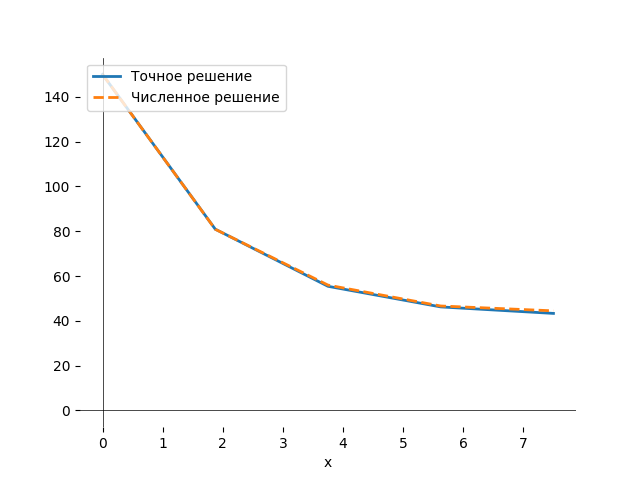
\includegraphics[scale=0.8]{1.png}
        \end{center}

        \item Для кубического элемента:
    \end{enumerate}
\end{enumerate}
        \[
        \begin{bmatrix}
        1,0000 & 0,0000 & 0,0000 & 0,0000 & 0,0000 & 0,0000 & 0,0000 & 0,0000 \\
        -271,1206 & 742,3224 & -459,2257 & 76,3811 & 0,0000 & 0,0000 & 0,0000 & 0,0000 \\
        76,3811 & -459,2257 & 742,3224 & -271,1206 & 0,0000 & 0,0000 & 0,0000 & 0,0000 \\
        -16,9388 & 76,3811 & -271,1206 & 482,2614 & -271,1206 & 76,3811 & -16,9388 & 0,0000 \\
        0,0000 & 0,0000 & 0,0000 & -271,1206 & 742,3224 & -459,2257 & 76,3811 & -16,9388 \\
        0,0000 & 0,0000 & 0,0000 & 76,3811 & -459,2257 & 742,3224 & -271,1206 & 0,0000 \\
        0,0000 & 0,0000 & 0,0000 & 0,0000 & 76,3811 & -271,1206 & 241,1307 & 0,0000 \\
        0,0000 & 0,0000 & 0,0000 & -16,9388 & 76,3811 & -271,1206 & 241,1307 & 0,0000 \\
        \end{bmatrix}
        \]
        
        Вектор правой части \( \mathbf{f}^T \) равен:
        \[
        \begin{bmatrix}
        150,0000 & 3534,2917 & 3534,2917 & 2356,1945 & 3534,2917 & 3534,2917 & 1178,0972
        \end{bmatrix}
        \]
        
        Решение системы:
        \[
        \begin{array}{|c|c|c|}
        \hline
        \text{№ узла} & \text{Температуры, полученные МКЭ} & \text{Точные значения температуры} \\
        \hline
        1 & 150,00 & 150,00 \\
        2 & 96,83 & 80,90 \\
        3 & 69,51 & 55,40 \\
        4 & 55,52 & 55,40 \\
        5 & 48,42 & 46,20 \\
        6 & 45,15 & - \\
        7 & 44,22 & 43,30 \\
        \hline
        \end{array}
        \]

        Сравнение численного и аналитического решения:
        \begin{center}
            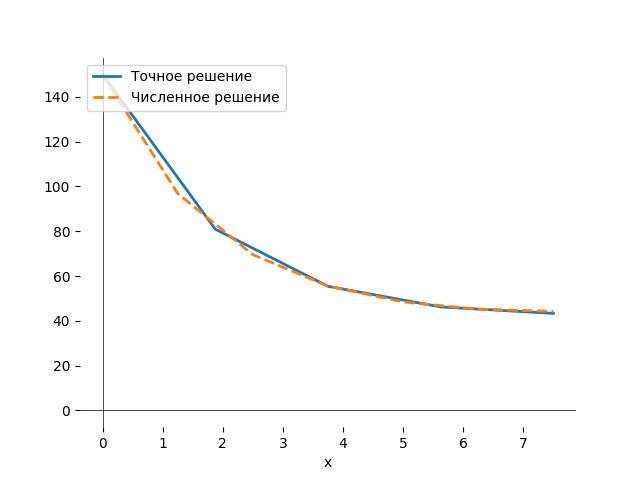
\includegraphics[scale=0.8]{2.png}
        \end{center}
\end{document}